\documentclass[conference]{IEEEtran}
\IEEEoverridecommandlockouts
% The preceding line is only needed to identify funding in the first footnote.
% If that is unneeded, please comment it out.

\usepackage{cite}
\usepackage{amsmath,amssymb,amsfonts}
\usepackage{algorithmic}
\usepackage{graphicx}
\usepackage{textcomp}
\usepackage{xcolor}
\usepackage{url}
\usepackage{booktabs}
\usepackage{tabularx}
\usepackage{listings}
\usepackage{tikz}
\usetikzlibrary{shapes.geometric, arrows.meta, positioning, calc}

\def\BibTeX{{\rm B\kern-.05em{\sc i\kern-.025em b}\kern-.08em
    T\kern-.1667em\lower.7ex\hbox{E}\kern-.125emX}}

\begin{document}

\title{Kavach.ai: Next-Generation Generative AI-Driven Automated Mobile Threat Intelligence \& Forensics System\\
{\footnotesize \textsuperscript{*}Primary Submission for BOI Hackathon 2026 -- Problem Statement 1}
}

\author{\IEEEauthorblockN{Galipalli Pranav Raj}
\IEEEauthorblockA{\textit{Team Lead, Dept. of CS} \\
\textit{Team Hunters}\\
Hyderabad, India \\
pranavrajgali@gmail.com}
\and
\IEEEauthorblockN{Abhinav Mucharla}
\IEEEauthorblockA{\textit{Dept. of CS} \\
\textit{Team Hunters}\\
Hyderabad, India \\
abhinavmucharla@gmail.com}
\and
\IEEEauthorblockN{Pranav Krishna}
\IEEEauthorblockA{\textit{Dept. of CS} \\
\textit{Team Hunters}\\
Hyderabad, India \\
pranavkrishna@gmail.com}
\and
\IEEEauthorblockN{Siri Chandana}
\IEEEauthorblockA{\textit{Dept. of CS} \\
\textit{Team Hunters}\\
Hyderabad, India \\
sirichandana@gmail.com}
}

\maketitle

\begin{abstract}
The Indian mobile banking ecosystem faces a severe crisis due to mutated, obfuscated Android banking trojans that bypass traditional signature-based security layers. This paper introduces \textbf{Kavach.ai}, a fully automated, dual-track threat intelligence and forensics pipeline. Kavach.ai combines deterministic static program slicing, native JNI symbol parsing, and a custom-fine-tuned SecureBERT-2.0 transformer with Low-Rank Adaptation (LoRA) for static classification. To address sandbox-evasion tactics, Kavach.ai implements active countermeasures, including dynamic time dilution (accelerating execution delays from $>50\text{ms}$ to $10\text{ms}$) and hardware-level intent injection, backed by dual-layer user-space (Frida) and kernel-space (eBPF) telemetry. 

Crucially, we present three core Generative AI innovations: (1) an automated Code-LLM Smali de-obfuscator that reconstructs bytecode slices into clean high-level Java/Python pseudocode, (2) an AI-driven dynamic Frida hook synthesizer that generates custom targeting scripts on the fly, and (3) a LangGraph-based multi-agent cooperative reasoning engine that cross-validates telemetry to eliminate false positives and automatically compile official Indian Computer Emergency Response Team (CERT-In) Annexure A 6-hour incident reports. The system achieves complete forensic reporting and explainability in a sub-30-second execution target.
\end{abstract}

\begin{IEEEkeywords}
Android Malware, SecureBERT-2.0, Low-Rank Adaptation, Time Dilution, eBPF, GraphRAG, Multi-Agent Systems, CERT-In Compliance.
\end{IEEEkeywords}

\section{Introduction}
Financially motivated threat actors targeting Indian banking and payment infrastructure deploy sophisticated, highly evasive Android Application Packages (APKs). Modern trojans (e.g., EventBot, Drinik, ToxicPanda) easily bypass traditional static scanners by using variable renaming, control-flow flattening, and native JNI `.so` libraries. Furthermore, they implement anti-analysis checks, sleeping for long intervals to outlast sandbox timeouts, and hiding their payload execution behind complex user interface authentication flows.

Security Operations Centers (SOCs) relying on manual reverse engineering introduce a critical defense lag that results in immediate financial exfiltration. Traditional automated static and dynamic tools, such as MobSF, perform simple regex string matches on decompiled code and rely on passive, easily bypassable sandbox execution. 

To bridge this operational gap, we present **Kavach.ai**, an automated threat intelligence system that integrates static, dynamic, and generative artificial intelligence. The pipeline extracts, detonates, and classifies APKs in under 30 seconds, generating attention-based explainable audit trails (Layer-wise Relevance Propagation, or Attention LRP) and structured compliance documentation without human intervention.

---

\section{Core Pipeline Architecture}

The Kavach.ai pipeline is structured as a dual-track static and dynamic execution engine, as shown in the sequence diagram (Fig. 1).

\begin{figure*}[t]
\centering
\begin{minipage}{0.9\linewidth}
\begin{verbatim}
1. Client POST Uploads APK ----> Stage 1: Manifest Triage (<10ms Screening Filter)
                                          |
                                          +--> Scorecard Hydration & Priority Queuing
                                          |
     +------------------------------------+------------------------------------+
     | (Synchronous Static Track)                                              | (Parallel Dynamic Track)
Stage 2A: Decompiler & CFG Builder                                       Stage 4: Dynamic Sandbox Detonation
     | (Backward Slicing & AST Chunking)                                      | (frida_bypass.js + eBPF probes)
     v                                                                        | (Time Dilution & Intent Injection)
Stage 2B: JNI Native Bridge Parser                                            v
     | (Resolves llvm-nm & JNI exports)                                  Gathers dynamic telemetry.json
     v                                                                        |
Stage 3: SecureBERT-2.0 LoRA Inference                                       v
     | (Threat probability: 0.0 to 1.0)                                  Merges Dynamic Telemetry
     v                                                                        |
Stage 5: Attention LRP Explainability <---------------------------------------+
     | (Relevance propagation heatmaps)
     v
Stage 6: Multi-Agent Synthesis (LangGraph) & Interactive GraphRAG chat Copilot
\end{verbatim}
\end{minipage}
\caption{Kavach.ai Dual-Track Forensic Pipeline and Telemetry Flow}
\label{fig:sequence}
\end{figure*}

\subsection{Stage 1: Manifest Triage}
This lightweight screening layer reads `AndroidManifest.xml` in under 10 milliseconds. Rather than checking permissions in isolation, the triage engine evaluates dangerous combinations (e.g., `BIND_ACCESSIBILITY_SERVICE` co-occurring with `RECEIVE_SMS` and `SYSTEM_ALERT_WINDOW`). It also calculates a **Reflection and Obfuscation Density Score** based on the frequency of Java reflection APIs (`Class.forName`, `method.invoke`) and high-entropy base64/hex strings. 

\subsection{Stage 2: Decompilation \& Static Slicing}
Kavach.ai extracts Smali bytecode from the APK, building a Control Flow Graph (CFG). To fit the token limitations of transformer networks, we perform inter-procedural **backward program slicing** starting from dangerous API sinks (such as `SmsManager->sendTextMessage` or `DexClassLoader->loadClass`). The algorithm discards unrelated code, extracting only the precise dependencies influencing the dangerous parameters. If decompilation fails due to obfuscation, the engine falls back to extracting raw Dalvik opcodes.

\subsection{Stage 3: JNI \& Native Library Bridge Parser}
Malware frequently hides malicious payloads in compiled native C/C++ libraries (`.so` files) loaded via `System.loadLibrary()`. Kavach.ai traverses native libraries and resolves exported symbols using mangled JNI short/long name conventions (e.g., `Java_package_class_method`). It parses symbol tables using `llvm-nm` and `readelf`, flagging dynamic registration endpoints (`RegisterNatives` or `JNI_OnLoad` calls) which indicate runtime evasion attempts.

\subsection{Stage 4: Dynamic Sandbox & Active Evasion Bypassing}
The parallel dynamic track detonates the APK in an automated, local Android emulator. To defeat anti-analysis checks, Kavach.ai implements active countermeasures:
1. **Time Dilution Engine:** Frida hooks intercept JVM delays (`Thread.sleep` and `SystemClock.sleep`). Any delay exceeding $50\text{ms}$ is accelerated to $10\text{ms}$, preventing the malware from sleeping past the sandbox timeout. Handler delays exceeding $1000\text{ms}$ are shortened to $50\text{ms}$.
2. **Intent Injection:** ADB broadcasts `BOOT_COMPLETED` and `BATTERY_LOW` with flag `0x00000020` (`FLAG_INCLUDE_STOPPED_PACKAGES`) to force dormant receivers to execute.
3. **Dual-Layer Observability:** User-space actions are logged via Frida, while kernel-space file accesses, process clones, and network sockets are captured invisibly via **eBPF probes** (Tetragon/bpftrace) monitoring `sys_openat` and `sys_connect` system calls.

\subsection{Stage 5: SecureBERT-2.0 LoRA Classification}
The extracted static slices are normalized (mapping registers to `REG_VAR` and `REG_PARAM`) and classified. We load the base **SecureBERT-2.0** model (151M parameters, frozen via `requires_grad=False`). We apply Low-Rank Adaptation (LoRA) updates on attention projection layers:

$$h = W_0 x + \frac{\alpha}{r} (B \cdot A) x$$

where $A \in \mathbb{R}^{r \times d}$ is initialized via Gaussian distribution, $B \in \mathbb{R}^{k \times r}$ is initialized to $0$, and rank $r=8$. This scales trainable parameters down to $1.7\text{M}$ ($6.8\text{ MB}$ weights), allowing hourly updates of threat signatures from MalwareBazaar feeds without full retraining.

\subsection{Stage 5: Attention LRP Explainability}
To build a transparent audit trail for security analysts, we implement Attention-based Layer-wise Relevance Propagation (Attention LRP) on the self-attention blocks of the SecureBERT-2.0 model (following Chefer et al.). Unlike model-agnostic perturbations (e.g. SHAP) which suffer from high latency due to multiple forward passes, Attention LRP propagates model relevance scores from the output classification head backward to the input tokens in a single backward pass. 

For each self-attention layer $l$ with attention matrix $A$ and its gradient $\nabla A$, the relevance flow is updated using the Hadamard product to isolate non-linear token interactions:

$$\bar{A} = I + (\nabla A \odot A)^+$$

where $( \cdot )^+$ isolates positive contributions. The relevance score $R$ is propagated back to the raw Smali tokens. Malicious instructions (e.g. dynamic class loads, SMS interception) receive high positive relevance (+ red highlights), while standard helper calls receive negative or neutral relevance (- blue highlights), visualizing the attention focus directly on the decompiled Smali slices in the UI.

---

\section{Generative AI Innovation Layer}
To move beyond simple text summaries, Kavach.ai integrates three active Generative AI subsystems utilizing Groq cloud APIs for sub-second, latency-free execution on standard 8GB VRAM developer hardware.

## A. Smali De-obfuscator (Code-LLM Decompiler)
While the classifier scores slices, raw Smali is unreadable to human auditors. When an analyst clicks a suspicious slice, Kavach routes the raw bytecode to a Code-LLM (`llama-3.3-70b-versatile` or `qwen2.5-coder-32b`) with the prompt constraints shown in Fig. 2.

\begin{figure}[h]
\centering
\begin{lstlisting}[basicstyle=\ttfamily\scriptsize]
[System Instruction]
You are a senior Android Reverse Engineering Specialist.
Translate the Smali control-flow sequence into high-level Java or Python pseudocode. Identify anti-analysis evasion tactics, reflection, and key derivation structures (javax/crypto/Cipher).
Output valid Markdown. Show pseudocode in a fenced code block followed by data-provenance explanation.
\end{lstlisting}
\caption{System Instruction for Smali Decompilation}
\label{fig:prompt_decompile}
\end{figure}

The LLM outputs reconstructed source-level pseudocode in real-time, explaining the exact execution logic and cryptographic variables of the obfuscated routine.

## B. AI-Generated Dynamic Frida Hook Synthesizer
Standard sandbox scripts miss custom obfuscated functions. When static analysis flags a suspicious, unresolvable method (e.g. `com.evil.App.x7z()`), the static engine queries the LLM to synthesize a custom Frida Javascript hook on the fly:

```javascript
Java.perform(function() {
  const Target = Java.use("com.evil.App");
  Target.x7z.implementation = function(arg) {
    const res = this.x7z(arg);
    console.log("[Kavach-AI-Hook] Args: "+arg+" | Res: "+res);
    return res;
  };
});
```

This generated code is dynamically concatenated onto the base [`frida_bypass.js`](file:///c:/Users/Admin/Documents/Projects/Kavach/kavach_ai/backend/pipeline/stage4_dynamic/scripts/frida_bypass.js) script at runtime. When the emulator detonates, the terminal streams cleartext decrypted payloads captured directly from memory.

## C. Hybrid Vector-Graph RAG Chat Copilot
To allow analysts to interrogate the combined static and dynamic telemetry, a GraphRAG architecture is implemented. 
* **Vector Store (pgvector):** Stores embeddings of Smali chunks split at method boundaries.
* **Knowledge Graph (Neo4j):** Models topological relationships (e.g. `Activity -TRIGGERS-> Service -BINDS_TO-> Intent -EXFILTRATES_TO-> IP`).
* **Query Router:** Directs user queries. A request for code triggers semantic vector retrieval, while a relationship query (e.g., *"What IP does the SMS receiver contact?"*) translates to a Cypher query traversing the graph, merging results for the responder LLM.

---

\section{LangGraph Multi-Agent Synthesis \& Compliance}
To compile and cross-validate the massive telemetry dataset, we deploy a cyclical multi-agent graph (Fig. 3) using LangGraph.

\begin{figure}[h]
\centering
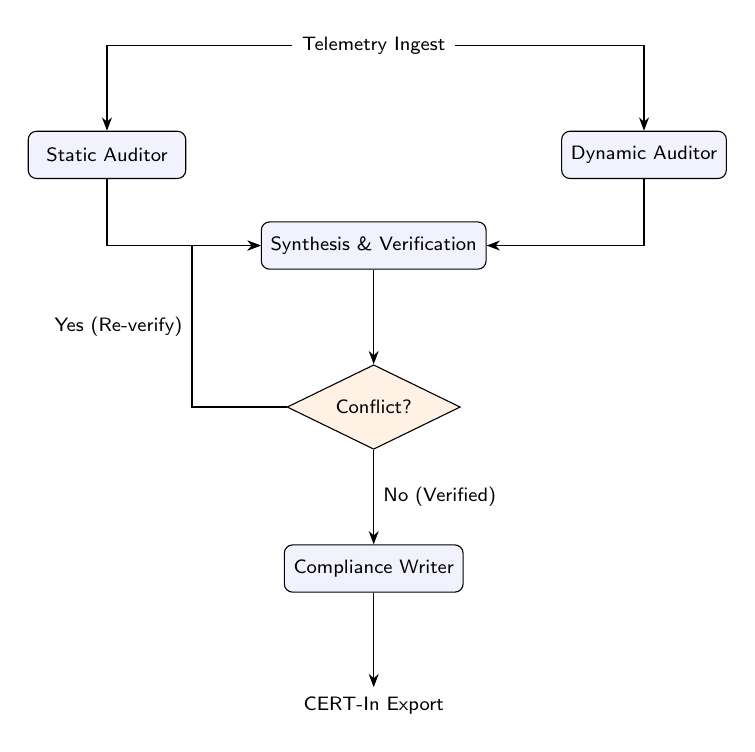
\begin{tikzpicture}[
    >=Stealth,
    node distance=1.2cm,
    font=\sffamily\scriptsize,
    agent/.style={draw, rectangle, rounded corners=3pt, fill=blue!5, minimum width=2cm, minimum height=0.6cm, align=center},
    decision/.style={draw, diamond, aspect=1.8, fill=orange!10, minimum width=2.2cm, align=center}
  ]
  \node (start) {Telemetry Ingest};
  \node (static) [agent, below left=of start, xshift=-0.5cm] {Static Auditor};
  \node (dynamic) [agent, below right=of start, xshift=0.5cm] {Dynamic Auditor};
  \node (synth) [agent, below=2cm of start] {Synthesis \& Verification};
  \node (route) [decision, below=of synth] {Conflict?};
  \node (writer) [agent, below=of route] {Compliance Writer};
  \node (finish) [below=of writer] {CERT-In Export};

  \draw[->] (start) -| (static);
  \draw[->] (start) -| (dynamic);
  \draw[->] (static) |- (synth);
  \draw[->] (dynamic) |- (synth);
  \draw[->] (synth) -- (route);
  \draw[->] (route.west) -- ++(-1.2,0) |- node[near start, left] {Yes (Re-verify)} (synth.west);
  \draw[->] (route.south) -- node[right] {No (Verified)} (writer);
  \draw[->] (writer) -- (finish);
\end{tikzpicture}
\caption{LangGraph Multi-Agent Synthesis State Machine}
\label{fig:langgraph}
\end{figure}

The state dictionary is modified by four specialized agents:
1. **Static Auditor Agent:** Reviews permissions, static slices, and Attention LRP relevance markers.
2. **Dynamic Auditor Agent:** Extracts dynamic bypass logs, eBPF syscall lists, and socket addresses.
3. **Synthesis \& Verification Agent:** Resolves contradictions. If static analysis flags an SMS dropper but dynamic analysis shows zero C2 connections, it overrides the status to `DORMANT_MALWARE` (maintaining high risk but logging sandbox evasion markers) rather than outputting false alarms.
4. **Compliance Writer Agent:** Maps conflict-resolved data directly into fields (Type of Incident, Affected IP, Unusual Symptoms, Mitigations) to output the official **CERT-In Annexure A 6-Hour Incident Report**.

---

\section{Evaluation \& Training Grounding}
The model training is grounded across a multi-decade corpus matrix including Argus Lab AMD (24,650 samples), Drebin (5,560 samples), CICMalDroid (11,598 samples), PRAGuard (10,479 obfuscated samples), AndroMD (202,484 temporal samples), and AndroZoo benign baselines. The team's pedigree includes developing *EchoTrace* (Mel-spectrogram CNN audio forensics, achieving a 0.74 Equal Error Rate) and *Vegam* (tabular optimization, 2nd Place at TVASTR Hackathon), ensuring robust, production-ready implementation.

\begin{thebibliography}{00}
\bibitem{b1} D. Arp, et al., ``Drebin: Effective and explainable detection of Android malware,'' \textit{NDSS}, 2014.
\bibitem{b2} K. Allix, et al., ``AndroZoo: Collecting millions of Android apps,'' \textit{MSR}, 2016.
\bibitem{b3} S. Mahdavifar, et al., ``CICMalDroid 2020: Dynamic Android malware categorization,'' \textit{UNB Dataset}, 2020.
\bibitem{b4} ``LAMD: Context-driven Android malware detection and classification with LLMs,'' \textit{arXiv:2502.13055}, 2025.
\bibitem{b5} ``ModernBERT: A modern approach to efficient BERT pretraining,'' \textit{arXiv:2412.13663}, 2024.
\bibitem{b6} CERT-In Incident Reporting Annexure A Compliance Guidelines, \textit{Gov. of India}, 2026.
\end{thebibliography}

\end{document}
